
\documentclass[class=article,crop=false]{standalone}
\usepackage{pacco}
\begin{document}
\section{L\'evy processes}
\textbf{L\'evy processes} were introduced in the 1930's by Paul L\'evy and Bruno De Finetti, one of the fathers of Bayesian Statistics. These processes have important applications to mathematical finance, mathematical biology and nonparametric Bayesian inference.
\begin{definition}
		A random variable $Y$ is said to be \textbf{infinitely divisible} (I.D.) if $\forall n \in \N$ there are $Y_i^{(n)}\; i.i.d.$ such that
	\[
	Y\stackrel{d}{=}Y_1^{(n)}+\ldots+Y_n^{(n)}
	\]
	i.e. $Y$ can be rewritten as sum of an arbitrary number $n$ of $i.i.d.$ random of variables.
\end{definition}
\begin{example}
	\begin{itemize}
		\item if \[
		Y\sim\text{Pois}(\lambda)\qquad:\qquad Y_i^{(n)}\stackrel{i.i.d.}{\sim}\text{Pois}\left(\frac{\lambda}{n}\right)
		\]
		by properties of the Poisson distribution, we know that
		\[\sum_{i=1}^{n}Y_i^{(n)}\sim \text{Pois}\left(\sum_{i=1}^{n}\frac{\lambda}{n}\right)=\text{Pois}(\lambda);\]
		\item If \[
		Y\sim\N(m,s^2)\qquad:\qquad Y_i^{(n)}\stackrel{i.i.d.}{\sim}N\left(\frac{m}{n},\frac{s^2}{n}\right)
		\]
		then $\sum_{i=1}^{n}Y_i^{(n)}\sim N(n,s^2)$;
		\item if \[
		Y\sim\Gamma(\alpha,\beta)\qquad:\qquad Y_i^{(n)}\stackrel{i.i.d.}{\sim}\Gamma\left(\frac{\alpha}{n},\beta\right)
		\]
		then $\sum_{i=1}^{n}Y_i^{(n)}\sim \Gamma(\alpha,\beta)$.
	\end{itemize}
\end{example}
A single way to establish I.D. is using $\ev{\exp^{iuk}}$. Take, for example, $Y\sim\text{Pois}(\lambda)$.
\begin{align*}
	\ev{e^{iuY}}&=\sum_{k\geqslant0}\exp^{iuk}\lambda^k\frac{e^{-\lambda}}{k!}\\
	&=e^{-\lambda}\sum_{k\geqslant0}\frac{\left(\lambda\exp^{iu}\right)^k}{k!}\\
	&=e^{-\lambda}e^{\lambda e^{iu}}\\
	&=e^{-\lambda(1-e^{iu})}
\end{align*}
So $Y_i^{(n)}\stackrel{i.i.d.}{\sim}\text{Pois}(\frac{\lambda}{n})$. Consider now
\begin{align*}
	\ev{\exp^{iu\sum_{i}^{n}Y_i^{(n)}}}&=\left[\exp^{-\frac{\lambda}{n}(1-\exp^{iu})}\right]^n\qquad \text{using }i.i.d.\text{ properties}\\
	&=e^{-\lambda(1-e^{iu})}.
\end{align*}
This suggests a strategy: we could define the \textbf{characteristic exponent} (c.e.) function of $Y$ to be:
\[
\psi(u)=-\log\ev{e^{iuY}}
\]
Then $Y$ is the I.D. if $\exists$ a random variable with c.e. $\psi^{(n)}$ such that:
\[\psi(u)=n\psi^{(n)}(u).\]
\begin{exercise}
	Check this fact for $N(m,s^2)$.
\end{exercise}
\begin{example}
	Consider $Y\sim\Gamma(\alpha,\beta)$. We have
	\[
	\ev(e^{iuY})=\frac{1}{\left(1-\frac{iu}{\beta}\right)^\alpha}=\left(\frac{1}{\left(1-\frac{iu}{\beta}\right)^\frac{\alpha}{n}}\right)^n
	\]
	which implies that 
	\[
	Y_i^{(n)}\stackrel{i.i.d.}{\sim}\Gamma(\frac{\alpha}{n},\beta)
	\]
\end{example}
\begin{definition}
	Let $N\sim$Poiss$(\lambda)$ and $Z_i\stackrel{i.i.d.}{\sim}F$ on $\R$ with $\mu_0$ mean at 0. The random variable
	\[Y\sum_{i=1}^{N}Z_i\qquad(Y=0 if N=0)\]
	is said to have \textbf{compound Poisson distribution}.
\end{definition}
Its characteristic function is:
\begin{align*}
	\ev{e^{iu\sum_{i=1}^{N}Z_i}}&=\ev{\ev{e^{iu\sum_{i=1}^{k}Z_i}|N=k}}\\
	&=\sum_{k\geqslant0}\frac{\lambda^ke^{-\lambda}}{k!}\ev{e^{iu\sum_{i=1}^{k}Z_i}}\\
	&=\sum_{k\geqslant0}\frac{\lambda^ke^{-\lambda}}{k!}\bigl[\underbrace{\ev{e^{iuZ_1}}}_{\int_\R e^{iux}F(\dif x)}\bigr]^k\\
	&=\exp^{-\lambda}e^{\lambda\int_\R e^{iux}F(\dif x)}\\
	&=\exp^{-\lambda\int_\R(1-e^{iux})F(\dif x)}.
\end{align*}
Now,
\begin{align*}
	\psi(u)&=\lambda\int_\R(1-e^{iux}F(\dif x))\begingroup\color{red}\cdot\frac{n}{n}\endgroup\\
	&=n\underbrace{\frac{\lambda}{n}\int_\R(1-e^{iux})F(\dif x)}_{\psi^{(n)}(u)}.
\end{align*}
So $Y$ is I.D. such that \[Y=\sum_{i=1}^{N}Z_i\stackrel{d}{=}\sum_{j=1}^{n}Y_j^{(n)}\]
and we have
\[
Y_j^{(n)}=\sum_{i=1}^{N_j^{(n)}}Z-i,\qquad Z_i\stackrel{i.i.d}{\sim}F\text{ and }N_j^{(n)}\stackrel{i.i.d.}{\sim}\text{Poiss}\left(\frac{\lambda}{n}\right)
\]
Which is still a compounded Poisson with Poisson rate/mean $\frac{\lambda}{n}$.
\begin{theorem}
	\textbf{L\'evy-Khintchine formula}. A random variable on $\R$ with c.e. $\psi(u)$ is I.D. if and only if there exists:
	\begin{itemize}
		\item $\mu \in \R$;
		\item $\sigma\geqslant 0$;
		\item a measure $\pi$ on $\R\setminus\{0\}$ satisfying:
		\[\int_\R(\underbracket{1\wedge x^2}_{\mathclap{\min\{1,x^2\}}})\pi(\dif x)<\infty\]
		such that, $\forall u\in\R$,
		\[\psi(u)=i\mu u +\frac{1}{2}\sigma^2 u^2+\int_\R\left(1-e^{iux}+iux\mathbbm{1}_{(|x|<1)}\right)\pi(\dif x).\]
	\end{itemize}
\end{theorem}
This characterizes I.D. distributions:
\begin{itemize}
	\item $\pi$ is called \textbf{L\'evy intensity};
	\item $(\mu,\sigma,\pi)=(-m,s,0)$ is called \textbf{characteristic triplet}.
\end{itemize}
\begin{example}
	\begin{itemize}
		\item $(mu,\sigma,\pi)=(-m,s,0)$, i.e. $\pi\equiv0$:
		\[
		\psi(u)=-imu+\frac{1}{2}s^2u^2
		\]which is the c.e. of $N(m,s^2)$.
		\item $(\mu,\sigma,\pi)=(0,0,\lambda\delta_1)$:
		\begin{align*}
			\psi(u)&=\lambda\int_\R(1-e^{iux}+iux\underbracket{\mathbbm{1}_{(|x|<1)}}_{\mathclap{=0}})\delta_1(\dif x)\\
			&=\lambda\int_\R(1-e^{iux})\delta_1(\dif x)\\
			&=\lambda(1-e^{iu})
		\end{align*}which means that $Y\sim\text{Pois}(\lambda)$.
	\end{itemize}
\end{example}
The requirement \[\int_{\R}\min\{1,x^2\}\pi(\dif x)<\infty
\]
implies:
\begin{itemize}
	\item $\int_{|x|\geqslant1}\pi(\dif x)<\infty$: the mean must be finite in both tails of $\pi$;
	\item $\int_{|x|\geqslant1}x^2\pi(\dif x)<\infty\implies$we can have $\pi\left((-1,1)\right)=\infty$ as long as $x^2\pi(\dif x)$ is integrable around 0.
\end{itemize}
For instance, $\pi(\dif x)\approx\frac{1}{x}\dif x$ around 0 is allowed.
\begin{figure}[H]
	\centering
	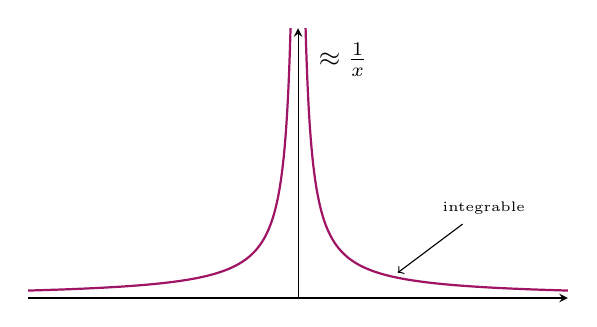
\begin{tikzpicture}
 \begin{axis}[
 	unit vector ratio*=1 1 1,
	axis lines = middle,
	ytick=\empty,
	xtick={0},
	xticklabel={0},
	scaled ticks = false,
	xmin = -6,
	xmax = 6,
	ymin = 0,
	ymax = 6,
	]
	\addplot[
	RedViolet, 
	thick, 
	domain = 0:20,
	samples=1000, 
	]
	{1/x};
	\addplot[
	RedViolet, 
	thick, 
	domain = 0:-20,
	samples=1000, 
	]
	{abs(1/x)};
	\node [anchor=west](source) at (axis cs:3,2) {\tiny integrable};
	\node (destination) at (axis cs:2,0.4){};
	\draw[->](source)--(destination);
	\node(lol) at(axis cs:1,5.3) {$\approx\frac{1}{x}$};
\end{axis}
\end{tikzpicture}
\end{figure}
\begin{definition}
		A L\'evy process on $\R$ is a continuous-time Càdlàg process $\{X(t),t\geqslant0\}$ such that:
	\begin{itemize}
		\item $X(0)=0$ a.s.;
		\item $X(s+t)-X(s)\stackrel{d}{=}X(u+t)-X(u)\qquad\forall s, u,t\geqslant0$: it has \sott{stationary increments};
		\item $X(s+t)-X(s)\independent\{X(u),u\leqslant s\}$: it has \sott{independent increments}.
	\end{itemize}
\end{definition}
\begin{example}
	Poisson process:
	\begin{itemize}
		\item $X(0)=0$ a.s.;
		\item $\underbracket{X(s+t)-X(s)}_{\mathclap{\independent s,X(s)}}\sim\text{Pois}(\lambda)$.
	\end{itemize}
	Brownian motion:
	\begin{itemize}
	\item $X(0)=0$ a.s.;
	\item $X(s+t)-X(s)\sim N(0,t)\independent s,X(s)$.
	\end{itemize}
\end{example}
\begin{definition}
	Let $N(t)$ be a rate $\lambda$ Poisson process and let $Y_i\stackrel{i.i.d.}{\sim}F$, independent of $N(t)$. Then
	\[X(t):=\sum_{i=1}^{N(t)}Y_i\qquad t\geqslant 0\] 
	is called \textbf{compound Poisson process}.
\end{definition}
\begin{exercise}
	Show that a CPP is also a L\'evy process and when $F=\delta_1$ it is a normal Poisson process.
\end{exercise}
\begin{figure}[H]
	\centering
	\begin{tikzpicture}%[scale=0.8]
	\begin{axis}[
		xlabel=\empty,
		x axis line style={->,opacity=100},
		ylabel=\empty,
		xmin=-1, xmax=100,
		ymin=-1, ymax=100,
		axis y line=left,
		y axis line style={->,opacity=100},
		ticks=none,
		axis x line*=bottom
		]
		\draw [RedViolet](0,0)--(30,0) node[circle,fill, pos=0,inner sep=2pt]{};
		\draw [RedViolet](30,60)--(50,60) node[circle,fill, pos=0,inner sep=2pt]{};
		\draw [RedViolet] (50,30)--(85,30) node[circle,fill, pos=0,inner sep=2pt]{};
		\draw [RedViolet] (85,80)--(100,80) node[circle,fill, pos=0,inner sep=2pt]{};
		\draw[dashed] (30,60)--(30,0);
		\draw[dashed] (50,60)--(50,30);
		\draw[dashed] (85,80)--(85,30);
		\begin{scope}[decoration=brace]
			\pgfdecorationsegmentamplitude=5pt
			\draw[decorate,black!80!black] (31,59)--(31,0) node[midway,right=\pgfdecorationsegmentamplitude,font=\tiny] {$Y_1$};
			\draw[decorate,black!80!black] (51,59)--(51,31) node[midway,right=\pgfdecorationsegmentamplitude,font=\tiny] {$Y_2$};
			\draw[decorate,black!80!black] (86,79)--(86,31) node[midway,right=\pgfdecorationsegmentamplitude,font=\tiny] {$Y_3$};
		\end{scope}
	\end{axis}
	\node[RedViolet,below right=0.1cm and 0.43cm, font=\tiny] (T) {Exp$(\lambda)$};
	\node[RedViolet,below right=0.1cm and 2.25cm, font=\tiny] (Te) {Exp$(\lambda)$};
\end{tikzpicture}
\end{figure}
\begin{exercise}
	Show that a finite sum of L\'evy processes is a L\'evy process.
\end{exercise}
\begin{example}
	$X(t)=\underbracket{X^{(1)}(t)}_{CP}+\underbracket{X^{(2)}(t)}_{BM}$
	\begin{figure}[H]
		\centering
		\documentclass{standalone}
\usepackage[framemethod=default]{mdframed}
\usepackage{tikz-cd}
\usepackage{tikz}
\usepackage[scr=rsfs]{mathalpha}
\usepackage[final]{pdfpages}
\usepackage{pgfplots,pgfplotstable}%per disegni
\usepgfplotslibrary{fillbetween}
\pgfplotsset{compat=1.16}
\usepackage{float}%per posizionamento disegni
\usetikzlibrary{shapes,patterns,arrows,positioning,calc,arrows.meta, bending, graphs, shadings,quotes,intersections,decorations}
\begin{document}

\pgfmathsetseed{654}
\begin{tikzpicture}
\begin{axis}[
  axis x line=center,
  axis y line=center,
  xtick=\empty,
  ytick=\empty,
  xlabel style={below right},
  ylabel style={above left},
  xmin=-10,
  xmax=160,
  ymin=-100,
  ymax=100]     
    \addplot[smooth,black,domain = 0:30.1,
        samples = 20,
        thick, name path=A] {(2*x-10)+7*rand};
        \addplot[smooth,black,domain = 29.9:80.1,
        samples =20,
        thick, name path=B] {(10*sin(8*(x+10))+10*rand+80};
        \addplot[smooth,black,domain = 79.9:150,
        samples = 25,
        thick,name path=C] {(-x+100)+10*rand};
    \path[name path=p1] (30,0)--(30,150);
    \path[name path=p2] (80,0)--(80,150);
    \fill [name intersections={of=A and p1}] (intersection-1) coordinate (a);
    \fill [name intersections={of=B and p1}] (intersection-1) coordinate (b);
    \fill [name intersections={of=B and p2}] (intersection-1) coordinate (c);
    \fill [name intersections={of=C and p2}] (intersection-1) coordinate (d);
    \draw[RedViolet,thick,dashed](a)--(b)node[midway,font=\tiny,right]{$Y_1$};
    \draw[RedViolet,thick,dashed](c)--(d)node[midway,font=\tiny,right]{$Y_2$};
\end{axis} %fashion
\end{tikzpicture}

\end{document}
	\end{figure}
	\begin{figure}[H]
		\centering
		\documentclass{standalone}
\usepackage{standtikz}
\begin{document}
\pgfmathsetseed{634}
\begin{tikzpicture}
\begin{axis}[
  axis x line=center,
  axis y line=center,
  xtick={0,15,30,45,135,150},
  xticklabels={$0$,$\frac{t}{n}$,$\frac{2t}{n}$,\empty,$\frac{(n-1)t}{n}$,$t$},
  ytick=\empty,
  xlabel style={below right},
  ylabel style={above left},
  xmin=-10,
  xmax=160,
  ymin=-10,
  ymax=100]     
    \addplot[smooth,black,domain = 0:150.1,
        samples = 30,
        thick, name path=A] {(0.6*x)-3+7*rand} node[pos=0.9,xshift=5pt,yshift=28pt,font=\scriptsize]{$X(t)$};
        \path (axis cs:0,0) 
        node [anchor=north west,yshift=-0.05cm] {0};
        \path[name path=tn](15,0)--(15,200);
        \path[name path=2tn](30,0)--(30,200);
        \path[name path=vuoto](45,0)--(45,200);
        \path[name path=nm1t](135,0)--(135,200);
        \path[name path=ciao](150,0)--(150,200);
        \fill[name intersections={of=A and tn}] (intersection-1) coordinate (a);
        \fill[name intersections={of=A and 2tn}] (intersection-1) coordinate (b);
        \fill[name intersections={of=A and vuoto}] (intersection-1) coordinate (c);
        \fill[name intersections={of=A and nm1t}] (intersection-1) coordinate (d);
        \fill[name intersections={of=A and ciao}] (intersection-1)coordinate (e);
        \draw[dotted,RedViolet!70!white,thick](15,0)--(a);
        \draw[dotted,RedViolet!70!white,thick](30,0)--(b);
        \draw[dotted,RedViolet!70!white,thick](45,0)--(c);
        \draw[dotted,RedViolet!70!white,thick](135,0)--(d);
        \draw[dotted,RedViolet!70!white,thick](150,0)--(e);
\end{axis} %fashion
\end{tikzpicture}

\end{document}
	\end{figure}
\end{example}
Let $X(t)$ be a L\'evy process and write:
\begin{align*}
	X(t)&=\underbracket{X\left(\frac{t}{n}\right)-X(0)}_{\mathclap{\textcolor{RedViolet}{Y_1^{(n)}}}}+\underbracket{X\left(\frac{2t}{n}\right)-X\left(\frac{t}{n} \right) }_{\mathclap{\textcolor{RedViolet}{Y_2^{(n)}}}}+\ldots+\underbracket{X\left(t\right)-X\left(\frac{(n-1)t}{n} \right) }_{\mathclap{\textcolor{RedViolet}{Y_n^{(n)}}}}\\
	&\implies Y_i^{(n)}\stackrel{i.i.d.}{\sim}\qquad\text{from indepedence and stationarity of increments}\\
	&=\sum_{i=1}^{n}Y_i^{(n)}
\end{align*}
So $X(t)$ is I.D..\par
Define 
\[\psi_t(u):=\log\ev{e^{iuX(t)}}.\]
as the c.e. of $X(t)$, from the sum:
\[\text{if }t=m\in\N\qquad\begin{cases}
	\psi_m=n\psi_{\frac{m}{n}} &n\in\N\\
	\psi_m=m\psi_1&n=m
\end{cases}\implies\psi_{\frac{m}{n}}=\frac{m}{n}\psi_1\]
that is, $\forall t$ rational 
\begin{equation*}
	\psi_t(u) = t \psi_1(u)
\end{equation*}
can be extended to $t \geqslant 0$. \\
So
\begin{equation*}
	\forall t \geqslant 0, \quad \psi_t(u) = t \psi_1(u)
\end{equation*}
So any L\'evy process is such that 
\begin{equation*}
	\mE[e^{i u X(t)}] = e^{- t \psi_1(u)}
\end{equation*}
and so it is characterised by its characteristic exponent at $t=1$; therefore, the L\'evy-Khintchine formula provides a characterisation of L\'evy processes.\\
\textbf{Example: Linear Brownian Motion}\\
\begin{equation*}
	d X(t) = m dt + s dB(t)
\end{equation*}
$\implies$
\begin{equation*}
	X(t) \sim N(mt, s^2 t)
\end{equation*}
$\implies$
\begin{align*}
	\mE[e^{i u X(t)}] &= e^{i (mt) u - \frac{1}{2}(s^2 t) u^2}\\
	&= \exp\Bigg\{{\underbracket{-t\underbrace{\left[-imu + \frac{1}{2}s^2 u^2\right]}_{\psi_1(u)}}_{t \psi_1(u)}}\Bigg\}
\end{align*}
So at time $t = 1$, we find the triplet 
\begin{equation*}
	(\mu, \sigma, \pi) = (-m, s,0)
\end{equation*}
This suggests:
\begin{itemize}
	\item $\mu$ describes a constant drift with slope $ -\mu$
	\item $\sigma$ describes a Brownian component with diffusion coefficient $\sigma^2$. 
\end{itemize}
\begin{example}
	CP:
	\begin{equation*}
		X(t) = \sum_{i=1}^{N(t)} Z_i
	\end{equation*}
	with 
	\begin{equation*}
		N(t) \sim Po(\lambda t)
	\end{equation*}
	and 
	\begin{equation*}
		Z_i \stackrel{i.i.d.} \sim F
	\end{equation*}
	\begin{equation*}
		\psi_t(u) = t \psi_1(u)  
	\end{equation*}
	implies that at time $t=1$ we get a CP R.V.
	\begin{equation*}
		X(1) = \sum_{i=1}^{N(1)} Z_i
	\end{equation*}
	where $N(1) \sim Po(\lambda)$.
	This implies that 
	\begin{equation*}
		\psi_1(u) = \lambda \int_\mR (1-e^{iux}) F(\dif x)
	\end{equation*}
	We compute 
	\begin{align*}
		\psi_1(u) &= \lambda \int_\mR \left(1-e^{iux} + \textcolor{RedViolet}{iux \mathbbm{1}_{(|x| < 1)}} - \textcolor{Dandelion!70!black}{iux \mathbbm{1}_{(|x| < 1)}}\right)F(\dif x) \\
		&= \int_\mR \left(1-e^{iux} + iux\mathbbm{1}_{(|x| < 1)}\right)\color{RedViolet}\underbracket{\color{black}\lambda F(\dif x)}_{\color{RedViolet}\pi(\dif x)}\color{black} - iu\color{RedViolet}\underbracket{\color{black} \lambda \int_{-1}^1 x F(\dif x)}_{\color{RedViolet} -\mu}
	\end{align*}
	so the triplet is 
	\begin{equation*}
		\mu= -\lambda \int_{-1}^1 x F(\dif x), \quad \sigma = 0, \quad \pi = \lambda F
	\end{equation*}
	So:
	\begin{equation*}
		\lambda = \int_\mR \pi(\dif x)
	\end{equation*}
	called \textbf{total mass of $\pi$}, is the Poisson rate for jump arrivals. \\
\end{example}
\begin{remark}
	The L\'evy intensity of a CP has a finite total mass by construction!
\end{remark}
The normalized $\pi$ yields 
\begin{equation*}
	F = \lambda^{-1} \pi
\end{equation*}
which gives the distribution of the jumps. \\
\includepdf[page=14,pagecommand={}]{../drawings/lec 17}
We talked about 
L\'evy processes, which are Markov processes with stationary and independent increments, characterized by the characteristic exponent at time $1$ through 
\begin{equation*}
	\psi_t(u) = t \psi_1(u)
\end{equation*}
\subsection{Subclasses of L\'evy Processes}
We introduced a different object, a compound Poisson process:
\begin{equation*}
	X(t) = \sum_{i=1}^N(t) Z_i
\end{equation*}
with $Z_i \stackrel{i.i.d.} \sim F$ with no mass at 0. in particular
$$N(t) \sim \text{Pois}(\lambda t)$$
The characteristic exponent of a generic compound Poisson process is 
\begin{equation*}
	\psi(u) = \lambda \int_\mR (1-e^{iux})F(\dif x)
\end{equation*}
\begin{remark}
	The $F$ is the distribution of the jump sizes and the lambda is the Poisson rate for jumps arrival. 
	$\lambda$ is the Poisson rate for jump arrivals
	\begin{equation*}
		\lambda = \int_\mR \pi(\dif x) < \infty
	\end{equation*}
	by construction. 
\end{remark}
We can add something to this.
If we add a drift to the compound Poisson process, we obtain a L\'evy process with characteristic exponent given by the sum of the exponents:
\begin{equation*}
	\lambda \int_\mR (1-e^{iux}) F(\dif x) - iub
\end{equation*}
where the drift is $bt$. \\
\begin{exercise}
	Show the triplet is $(\mu, \sigma, \pi)$, where
	\begin{itemize}
		\item $\sigma = 0$
		\item $\pi = \lambda F$
		\item $\mu = - (b+\lambda \int_{-1}^1 x F(\dif x))$
	\end{itemize}
\end{exercise}
\begin{example}
	In the previous lecture we had shown that a random variable $Y \sim \Gamma(\alpha, \beta)$ is infinitely divisible with characteristic function 
	\begin{equation}
		\label{star1}
		\frac{1}{(1-\frac{iu}{\beta})^\alpha} \underbrace{=}_{\text{Frullani integral}}\exp\left\{-\int_0^\iy(1-e^{iux})\alpha x^{-1} e^{-\beta x}\dif x\right\}
	\end{equation}
	Now, clearly, the integral becomes the characteristic exponent for the random variable since we can see
	\begin{equation*}
		\int_0^\iy(1-e^{iux}\alpha x^{-1} e^{-\beta x} = \psi(u)
	\end{equation*}
	and 
	\begin{equation*}
		\alpha x^{-1} e^{-\beta x}\dif x = \pi(\dif x)
	\end{equation*}
	We can add and subtract $iux 1_{(|x|<1)}$ and therefore, similarly to CP process, we get 
	\begin{equation*}
		\psi(u) = \int_0^\iy (1-e^{iux} - iux 1_{(|x|<1)}\pi(\dif x) - iu \int_0^1x \pi(\dif x)
	\end{equation*}
	From this, we can read the L\'evy triplet 
	\begin{equation*}
		\mu = - \int_0^1x \pi(\dif x),  \quad \sigma = 0, \quad \pi(\dif x) = \alpha x^{-1} e^{-\beta x}\dif x
	\end{equation*}
\end{example}
We can define basing on this a L\'evy process, then we want to understand what does is mean in terms of trajectories. We have infinitive mass around 0.  \\
We can use $\psi_t(u) = t \psi_1(u)$  to define a Gamma process as a L\'evy process with triplet as above, that is with exponent for $X(t)$ given by
\begin{equation*}
	\psi_t(u) = \int_0^\infty (1-e^{iux})dt x^{-1}e^{\beta x}\dif x
\end{equation*}
Now we can work background and fine the increments of the process. \\
So through \eqref{star1} we see that 
\begin{equation*}
	X(t) \stackrel{d}= X(s+t) - X(s) \sim Ga(\alpha t, \beta)
\end{equation*}
We would like to know the behaviour in terms of trajectories. \\
Note that:
\begin{itemize}
	\begin{minipage}{0.5\textwidth}
		\item for $x \ra \infty, \pi(\dif x) \approx e^{-\beta x} $ is integrable \\$ \implies\pi((1,\infty)) < \infty$. 
	\end{minipage}
	\begin{minipage}{0.4\textwidth}
		\begin{figure}[H]
			\centering
			\documentclass{standalone}
\usepackage{standtikz}
\begin{document}
\begin{tikzpicture}[scale=0.6]
    \begin{axis}[
    xlabel=\empty,
                xtick={1},
                ytick=\empty,
                x axis line style={->,opacity=100},
                ylabel=\empty,
                xmin=0, xmax=5,
                ymin=0, ymax=2,
                axis y line=left,
                y axis line style={->,opacity=100},
                axis x line*=bottom
    ]\addplot[RedViolet, 
	thick, 
	domain = 1:20,
	samples=1000, 
 name path=iperboledemmerda
	]
	{1/x};
    \draw[black, dashed](1,0)--(1,1);
    \end{axis}
\end{tikzpicture}
\end{document}
		\end{figure}
	\end{minipage}\par
	\begin{minipage}{0.5\textwidth}
		\item for $x \ra 0^+$, $\pi(\dif x)  \approx \frac{1}{x}$ \\ $\implies \pi\left((0,1)\right)=\infty$: there is infinite mass in every neighbourhood of 0.
	\end{minipage}
	\begin{minipage}{0.4\textwidth}
		\begin{figure}[H]
			\centering
			\documentclass{standalone}
\usepackage{standtikz}
\begin{document}
\begin{tikzpicture}[scale=0.6]
    \begin{axis}[
    xlabel=\empty,
                xtick={1},
                ytick=\empty,
                x axis line style={->,opacity=100},
                ylabel=\empty,
                xmin=0, xmax=5,
                ymin=0, ymax=5,
                axis y line=left,
                y axis line style={->,opacity=100},
                axis x line*=bottom
    ]\addplot[RedViolet, 
	thick, 
	domain = 0:1,
	samples=100, 
 name path=iperboledemmerda
	]
	{1/x};
    \draw[black, dashed](1,0)--(1,1);
    \node[circle,anchor=west,font=\Large] at (2,2){$\infty$ mean};
    \draw[black,->,bend left](2,2) to [bend right](0.6,1.1);
    \end{axis}
\end{tikzpicture}
\end{document}
		\end{figure}
	\end{minipage}
        The requirement in the L\'evy–Khintchine formula 
\begin{equation*}
	\int_\mathbb{R} \min(1,x^2) \pi(\dif x) < \iy
\end{equation*}

is satisfied: around $0$ we have $\frac{x^2}{x}$. \\
Technically we have something legitimate that we do not understand:
since $\pi(\mathbb{R}_+)=\iy$ it is not a Compound Poisson.\\  
\end{itemize}
The Gamma process belongs to the following subclass of L\'evy processes.
\begin{definition}
	 A \textbf{subordinator} is a L\'evy process with almost surely non-decreasing sample paths, hence with triplet:
	\begin{itemize}
		\item $\mu \leq 0$ (so we have a non-negative drift $-\mu$);
		\item $\sigma = 0$ that is, there is no Brownian component (indeed, it couldn't have this component because of its oscillations); %non so se ho capito bene il discorso. 
		\item $\pi((-\infty,0]) = 0$, (se we only select positive jumps). 
	\end{itemize}
\end{definition}
\begin{remark}
	The Gamma process is gonna be used a lot in Bayesian Statistics where we will use it to create appropriate prior distributions. 
\end{remark}
We want to understand path properties when $\pi$ has total mass. We write a generic characteristic exponent as follows
\begin{equation*}
	\psi(u)  = \underbrace{i\mu u + \frac{1}{2}\sigma^2 u^2}_{\psi^{(1)}} + \underbrace{\int_{(-1,1)^c}(1-e^{iux})\pi(\dif x)}_{\psi^{(2)}} + \underbrace{\int_{(-1,1)}(1-e^{iux} + iux 1_{(|x|<1)})\pi(\dif x)}_{\psi^{(3)}}
\end{equation*}
$\psi^{(1)}$ is the exponent of a Brownian Motion
\begin{equation*}
	d X^{(1)}(t) = - \mu dt + \sigma dB(t) 
\end{equation*}
\begin{itemize}
	\item $\psi^{(1)}:$ is a linear BM
	\item $\psi^{(2)}:$ outside $(-1,1)$ $\pi$ has finite mass so $\psi^{(2)}$ can be written as
	\begin{equation*}
		\lambda_0 \int_{(-1,1)^C} (1-e^{iux}) F_0(\dif x)
	\end{equation*}
	with $\lambda_0 := \pi((-1,1)^C)$ and $F_0 : = \lambda_0^{-1} \pi |_{(-1,1)^C}$.\\ 
	We look outside a neighborhood of zero and then we can normalize measure and therefore we can have a compound Poisson. \\
	So $\psi^{(2)}$ corresponds to a CP process with $\lambda_0$ Poisson rate and $F_0$ distribution for jumps of size $|x|\geq 1$.
	\item $\psi^{(3)}:$ we can distinguish two cases
	\begin{enumerate}
		\item $\pi((-1,1)) < \infty$
		\begin{equation*}
			\int_{-1}^{+1}(1-e^{iux} + iux)\underbracket{\pi(\dif x)}_{\mathclap{\substack{<\infty\text{: we can split}\\ \text{the integral}}}} = u x \pi(\dif x)\underbracket{\int_{-1}^{+1}(1-e^{iux})\pi(\dif x)}_{C.P.} + \underbracket{iu \int_{-1}^{+1} x \pi(\dif x)}_{\text{drift}}
		\end{equation*}
		\item $\pi((-1,1)) = \infty$
		Jumps arrive at infinite rate (the total mass is infinite) but we cannot normalize $\pi$ to get the jump distribution. 
		So, the condition 
		\begin{equation*}
			\int_R \min(1,x^2) \pi(\dif x)<\iy
		\end{equation*}
		implies:
		\begin{itemize}
			\item "big jumps" (size greater or equal than $1$) arrive at finite rate $\pi((-1,1)^C) < \infty$ hence they occur finitely often in every bounded interval. 
			\item If $\pi((-1,1)) = \infty$, "small jumps" arrive at infinite rate (precisely given by that mass), hence they occur infinitely often in every bounded interval. 
		\end{itemize}
	\end{enumerate}
	Even if it seems that the trajectories are somewhere flat, they are not: there are infinite small jumps. The Gamma process only increases by jumps. The trajectory are nowhere continuous. Such a process is said to have \textbf{infinite activity}.  
\end{itemize} 
\begin{definition}
	A measure $N$ on a $\sigma$-finite measure space $(\mathbb{X}, \mathcal{X}, \mu)$ is said to be a \textbf{Poisson random measure} (PRM) with mean intensity measure $\mu$ if for mutually disjoint sets $A_1,\dots,A_k \in\mathbb{X} $
	$$\mathcal{N}(A_i) \stackrel{i.i.d.} \sim  P_0(\mu(A_i))$$
\end{definition} 
\begin{example}
	$\mathbb{X} = \mathbb{R}_+ \times \mR$
	\begin{figure}[H]
		\centering
		\documentclass{standalone}
\usepackage{standtikz}
\begin{document}
\begin{tikzpicture}
\begin{axis}[
    xlabel=\empty,
                xtick=\empty,
                ytick=\empty,
                x axis line style={->,opacity=100},
                ylabel=\empty,
                xmin=-1, xmax=5,
                ymin=-1, ymax=2,
                axis y line=left,
                axis lines=middle,
                y axis line style={->,opacity=100}]
                \node[fill,circle,inner sep=1.5pt]at(1,1){};
                \node[fill,circle,inner sep=1.5pt]at(1.9,-0.5){};
                \node[fill,circle,inner sep=1.5pt]at(3,1.6){};
                \node[fill,circle,inner sep=1.5pt]at(4.1,0.6){};
                \node[fill,circle,inner sep=1.5pt]at(3.5,-0.9){};
                \node[fill,circle,inner sep=1.5pt]at(0.5,-0.7){};
                \node[fill,circle,inner sep=1.5pt]at(0.2,1.5){};
                \node[fill,circle,inner sep=1.5pt]at(4.7,1.2){};
                \node[fill,circle,inner sep=1.5pt]at(2.6,1.1){};
                \draw[RedViolet](2.4,0.4)--(2.4,1.7) node[midway,left]{$A$};
                \draw[RedViolet](2.4,0.4)--(4.9,0.4);
                \draw[RedViolet](4.9,0.4)--(4.9,1.7);
                \draw[RedViolet](4.9,1.7)--(2.4,1.7);
\end{axis}
\end{tikzpicture}
\end{document}
	\end{figure}
	$N(A) \stackrel{i.i.d.} \sim Po(\mu(A))$. \\
	If $A = [s,t] x [a,b] $, $\mu = \text{Lebesgue measure} \times \pi$
	\begin{equation*}
		\mu(A) = \lambda(t-s) \int_a^bF(\dif x)
	\end{equation*}
	where $\pi = \lambda F$. 
\end{example}
\begin{proposition}
	 Let $N$ be a PRM on $[0,\infty) \times \mR$ with mean intensity $\mu=Leb \times \pi$, with $\pi$ finite on $\mR$ such that $\pi(\{0\}) = 0$. \\
	For any Borel set $B \in \mathcal{B}(\mR)$ 
	\begin{equation*}
		X_B(t):= \int_0^t \int_B x N(ds,\dif x) 
	\end{equation*}
	is a compound Poisson process with rate $\lambda_B:= \pi(B)$ and jump distribution $F_B = \lambda_B^{-1} \pi|_B$. 
\end{proposition}
\begin{example}
	Assume that $B = \mR$, $\pi$ is finite. Then, we can show that 
	\begin{equation*}
		N = \sum_{i \geq 1}1_{(s_i,Z_i)}
	\end{equation*}
	which gives us the random point configuration.\\
	This yields that 
	\begin{equation*}
		\int_0^t \int_B x \sum_{i \geq 1}1_{(s_i,Z_i)} (ds,\dif x) = \bigotimes
	\end{equation*}
	What we are saying is: we take the s and accumulate the x and the x is the second coordinate z. Sum up the second coordinate, that is sum up the heights of everything.
	$$\bigotimes = \sum_{i\geq1} Z_i 1_{(s_i \in [0,t], Z_i \in B)}$$
	The PRM is a random object which gives us the properties of the sample paths.\\
	We sum points heigth of every point $(S_i, Z_i) \in [0,t] \times B$ (if $B = \mR$, we sum all jumps sizes/points heights in $(0,t]$). 
\end{example}
If we now let, for general $\pi$ (so in every $[0,t] \times [0,\varepsilon]$ there could be infinitely many points).
\begin{align*}
	\varepsilon_m &= \frac{1}{x^m}, \quad m \geq 1\\
	B_m &= (-1, - \varepsilon_m] \cup [\varepsilon_m, 1)
\end{align*}
Set 
\begin{equation*}
	X^{(\varepsilon,m)}(t) := \underbrace{\int_0^t\int_{B_m} x N(ds,\dif x)}_{\text{CP since} \pi(B_m)<\iy} - \underbrace{t \int_{B_m}x\pi(\dif x)}_{\text{drift}}
\end{equation*}
which has exponent 
\begin{equation*}
	\psi^{(3,m)} = \int_{B_m}(1-e^{iux}) \pi(\dif x) + iu \int_{B_m} x \pi(\dif x)
\end{equation*}
informally, as $n \ra \infty$, we obtain the exponent we were looking for. \\
\begin{equation*}
	\psi^{(3)}= \int_{|x|<1}(1-e^{iux} + iux)\pi(\dif x)
\end{equation*}
More formally:
\begin{proposition}
	Let $X^{(3,m}$ be a L\'evy process with exponent $\psi^{(\varepsilon,m)}(CP + drift)$.\\
	As $m \ra \infty, X^{(3,m)} \stackrel{a.s.} \ra X^{(3)}$ uniformly over $[0,T]$, where $X^{(3)}$ is a L\'evy process with exponent $\psi^{(3)}$ and with at most countably-many discontinuities in every bounded interval.
\end{proposition}
If $C_n = [\frac{1}{2^n},\frac{1}{2^{n-1}}), B_m = \bigcup_{n = 1} ^ m C_n$:\\
\begin{figure}[H]
	\centering
	\documentclass{standalone}
\usepackage{standtikz}
\begin{document}
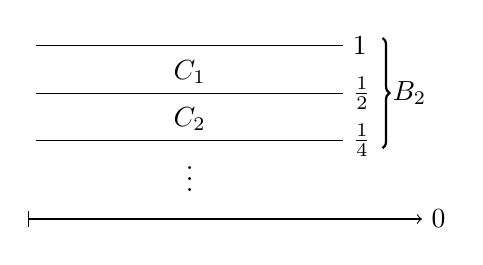
\begin{tikzpicture}[decoration=brace]
  \draw[|->,black] (0,0)--(5,0) node [anchor=west,pos=1]{0};
  \draw[black] (0.1,1)--(4,1) node [anchor=west,pos=1]{$\frac{1}{4}$}node[midway,anchor=south]{$C_2$} node[midway,anchor=north]{$\vdots$};
  \draw[black] (0.1,1.6)--(4,1.6) node [anchor=west,pos=1]{$\frac{1}{2}$} node[midway,anchor=south]{$C_1$};
  \draw[black] (0.1,2.2)--(4,2.2) node [anchor=west,pos=1]{1};
  \draw[black,decorate,thick] (4.5,2.3)--(4.5,0.9) node[anchor=west,midway]{$B_2$};
\end{tikzpicture}
\end{document}
\end{figure}
\begin{align*}
	\psi^{(\varepsilon,m)} &=\int_{B_m}(1-e^{iux}+iux)\pi(\dif x)=\\
	&=\sum_{n=1}^m[\lambda\underbracket{\int_{C_n}(1-e^{iux})F_n(\dif x)}_{C.P.}+ iu \lambda_n\underbracket{\int_{C_n}x F_n(\dif x)}_{\text{Drift}}]
\end{align*}
Hence the exponent of the process that converges to the limit process is given by a sum of cp processes whose jumps sizes are in disjoint intervals.
\begin{theorem}
	\enf{L\'evy-Ito decomposition}. Let $(\mu, \sigma, \pi)$ satisfy the conditions of the L\'evy-Kinthchine formula. \\
	Any L\'evy process $X$ is the superposition of three intependent L\'evy processes, such that 
	\begin{equation*}
		X = X^{(1)} + X^{(2)} + X^{(3)}
	\end{equation*}
	where 
	\begin{enumerate}
		\item $X^{(1)}$ is a linear Brownian Motion $dX^{(1)} = \mu dt + \sigma dB(t)$
		\item $X^{(2)}$ is a CP with jumps low
		\begin{equation*}
			F_0:=\lambda_0^{(-1)} \pi |_{(-1,1)^C}
		\end{equation*}
		and rate 
		\begin{equation*}
			\lambda_0 := \pi((-1,1)^C)
		\end{equation*}
		\item $X^{(3)}$ is the sum of countably-many CP processes with drift and jumps in $(-1,1)$. 
	\end{enumerate}
\end{theorem}
\begin{exercise}
	Verify superposition of CP and parameterisation for the Gamma process. 
\end{exercise}
 So the Gamma process has no Brownian component, $\pi$ was on $mR_+$ and there was no drift. Hence, it is a process which there are infintely - many jumps in every small bounded interval. \\
 \begin{figure}[H]
 	\centering
 	\begin{minipage}{.5\textwidth}
 		\centering
 		\includegraphics[page=11,scale=0.52,trim={4.3cm 7cm 4cm 5cm},clip]{../drawings/Lec 18.pdf}
 	\end{minipage}%
 	\begin{minipage}{.5\textwidth}
 		\centering
 		\includegraphics[page=12,scale=0.52,trim={4.3cm 7cm 4cm 5cm},clip]{../drawings/Lec 18.pdf}
 	\end{minipage}
 \end{figure}
 \begin{figure}[H]
 	\centering
 	\begin{minipage}{.5\textwidth}
 		\centering
 		\includegraphics[page=13,scale=0.52,trim={4.3cm 7cm 4cm 5cm},clip]{../drawings/Lec 18.pdf}
 	\end{minipage}%
 	\begin{minipage}{.5\textwidth}
 		\centering
 		\includegraphics[page=15,scale=0.52,trim={4.3cm 7cm 4cm 5cm},clip]{../drawings/Lec 18.pdf}
 	\end{minipage}
 \end{figure}
 \begin{figure}[H]
 	\centering
 	\includegraphics[page=14,scale=0.7,trim={4.3cm 12cm 4cm 5cm},clip]{../drawings/Lec 18.pdf}
 \end{figure}
 
\end{document}
